\chapter{Technical Evaluation}
As discussed in the Experiment Design and Implementation sections, each problem was run on both Hadoop and Stratosphere with a varying number of nodes. The same data was used for all of the experiments, and a runtime average was taken to provide the best possible indication of each tools performance.

This chapter provides a technical analysis of the results gained from experimentation, and relates them back to the hypothesis.

\section{Reverse Link Graph}

\subsection{Hadoop}
The Hadoop implementation of the Reverse Link Graph is important as a benchmark against which other experiments can be judged. The performance of Hadoop in MapReduce situations is a well-known quantity, as it is the most widely used data processing technology. This provides a clear metric against which the performance of Stratosphere can be evaluated, whilst also serving to illustrate how well Hadoop performs MapReduce tasks in comparison to non-MapReduce tasks.

\begin{figure}[H]
\centering
	\begin{tabular}{lrr}
		\toprule
		Number of Machines & Average Runtime & Standard Deviation \\
		\midrule

		2 & 430.60 & 144.20 \\
		4 & 274.60 & 41.72 \\
		6 & 211.20 & 31.91 \\
		8 & 172.40 & 15.70 \\
		10 & 173.40 & 3.28 \\
		\bottomrule
	\end{tabular}
	\caption{Hadoop Reverse Link Graph Raw Data}
\end{figure}

\begin{figure}[H]
	\centering
	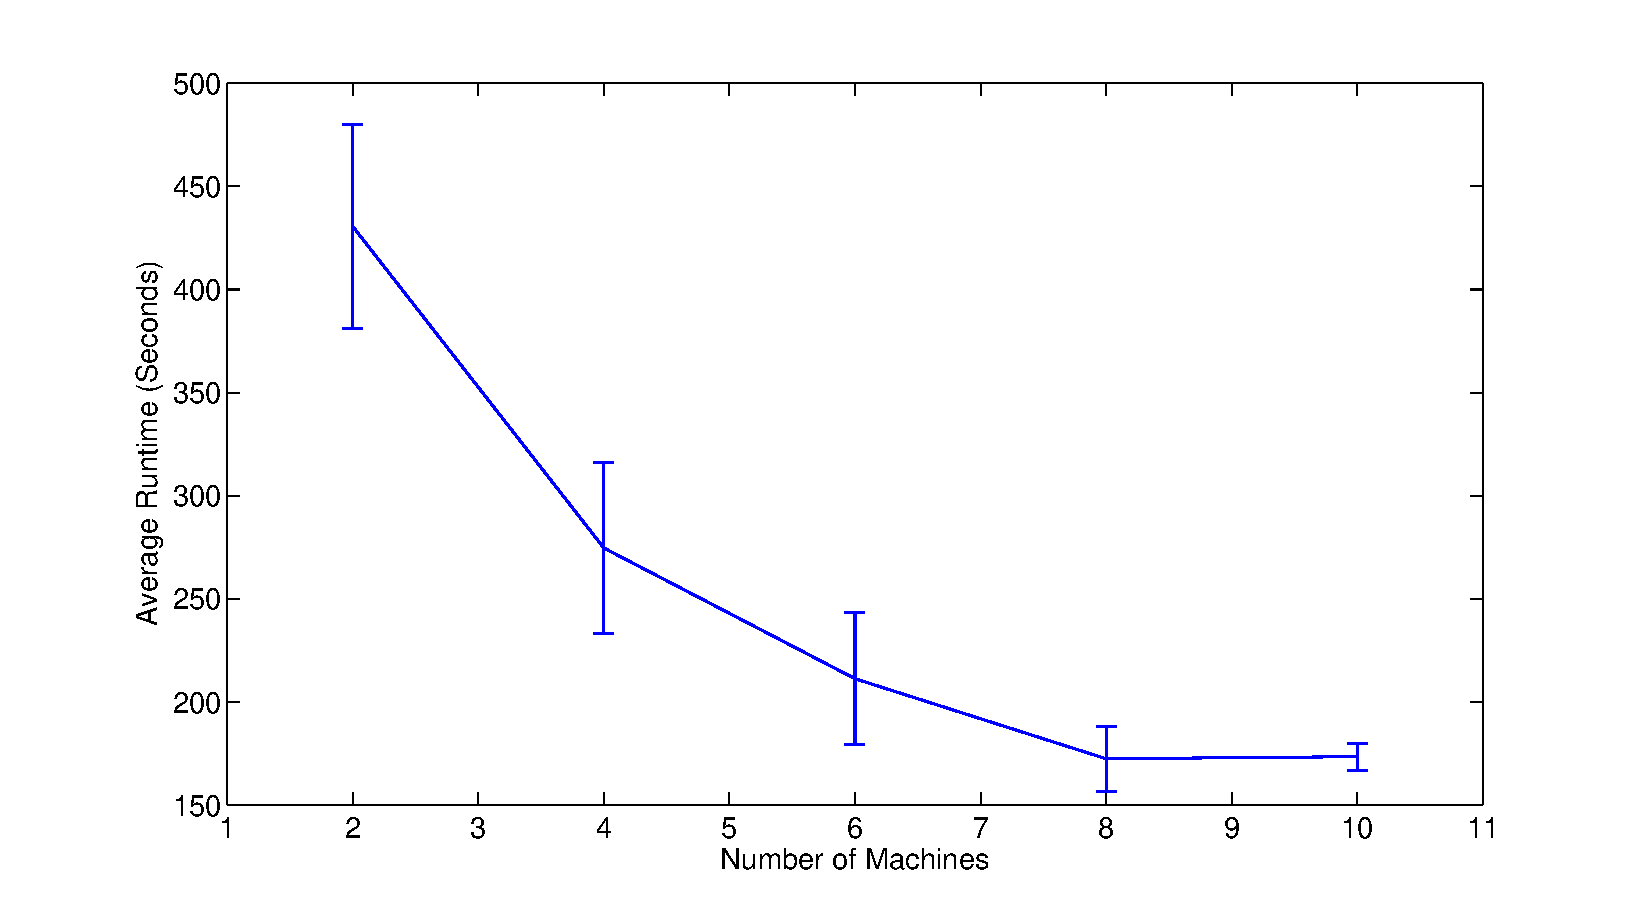
\includegraphics[scale=0.6]{resources/HadoopRLG.eps}
	\caption{Hadoop Reverse Link Graph Runtime}
	\label{hadoopRLGRuntime}
\end{figure}

The Hadoop implementation of the Reverse Link Graph problem shows the general properties expected from the data. As the number of nodes increases, the runtime decreases as having a larger amount of resources allows more work to be processed in parallel. This trend reverses when the experiment is executed on 10 machines. This typically indicates that a point has been reached where a problem no longer benefits from adding additional parallel resources, and it becomes more costly to run on a larger number of machines because of communications overhead. The impact of Amdahl's law \cite{amdahl1967validity} is not indicative of a problem with Hadoop, and is likely caused by the size of the data, as discussed in the Experiment Implementation section.

The expected trend of performing scaling near-linearly as the number of machines increases can be seen more clearly in figure \ref{hadoopRLGScalability}. This exhibits the expected behaviour that the runtime nearly halves as the number of machines is doubled. As expected, the runtime is not quite linear as there is some communications overhead added by adding more machines to the cluster. This reflects the change that can be seen in figure \ref{hadoopRLGRuntime} toward the end of the plot. Figure \ref{hadoopRLGScalability} does not show the more dramatic decrease in performance that can be seen when the experiment is run on 10 machines, as it only features the runtime for 2, 4 and 8 nodes. This effect would be shown if the experiment was performed on 16 nodes.

\begin{figure}[H]
	\centering
	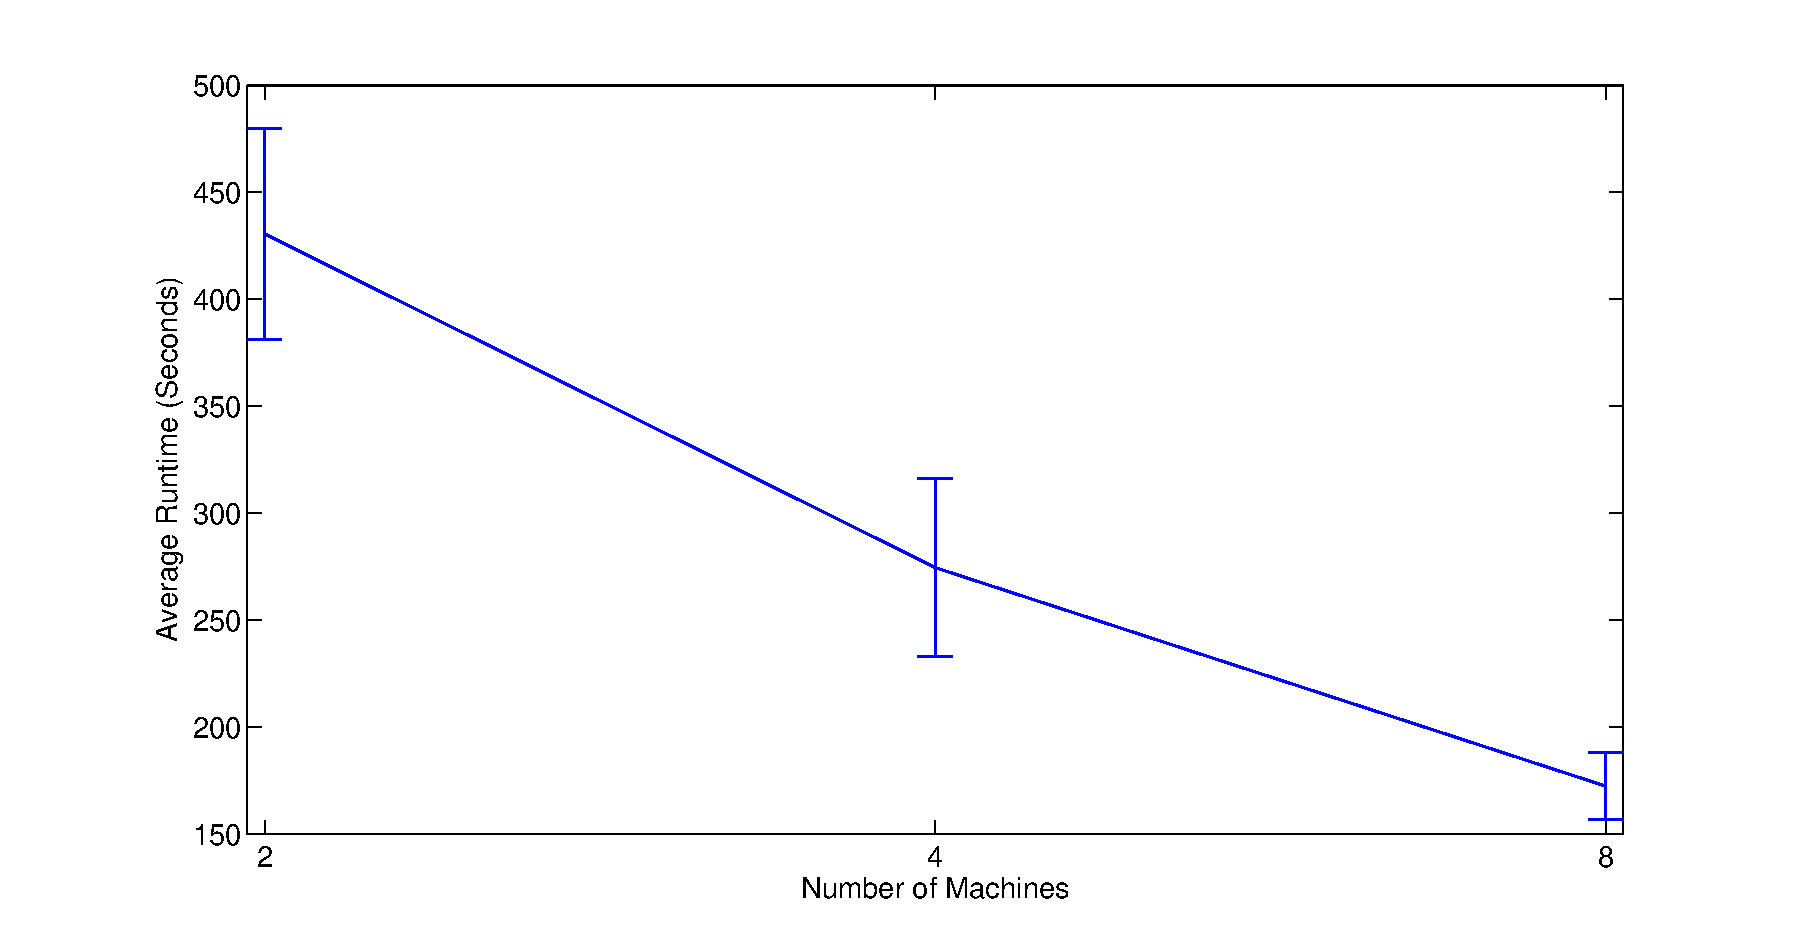
\includegraphics[scale=0.6]{resources/HadoopRLGScalability.eps}
	\caption{Logarithmic plot of Hadoop Reverse Link Graph Runtime}
	\label{hadoopRLGScalability}
\end{figure}

Another important factor of figure \ref{hadoopRLGRuntime} is the error bars, indicating the standard deviation of runtime. The standard deviation is initially fairly high, as the experiments take a (relatively) long time to run. As the number of machines increases, there becomes less room for error as the time taken is decreased. 

\subsection{Stratosphere}
The Stratosphere implementation of the Reverse Link Graph experiment allows a comparison of how well it can perform standard MapReduce tasks in comparison to Hadoop. 

\begin{figure}[H]
\centering
	\begin{tabular}{lrr}
		\toprule
		Number of Machines & Average Runtime & Standard Deviation \\
		\midrule

		2 & 144.20 & 1.92 \\
		4 & 92.20 & 2.04 \\
		6 & 72.00 & 1.87 \\
		8 & 62.20 & 3.63 \\
		10 & 59.40 & 3.28 \\
		\bottomrule
	\end{tabular}
	\caption{Stratosphere Reverse Link Graph Raw Data}
\end{figure}

\begin{figure}[H]
	\centering
	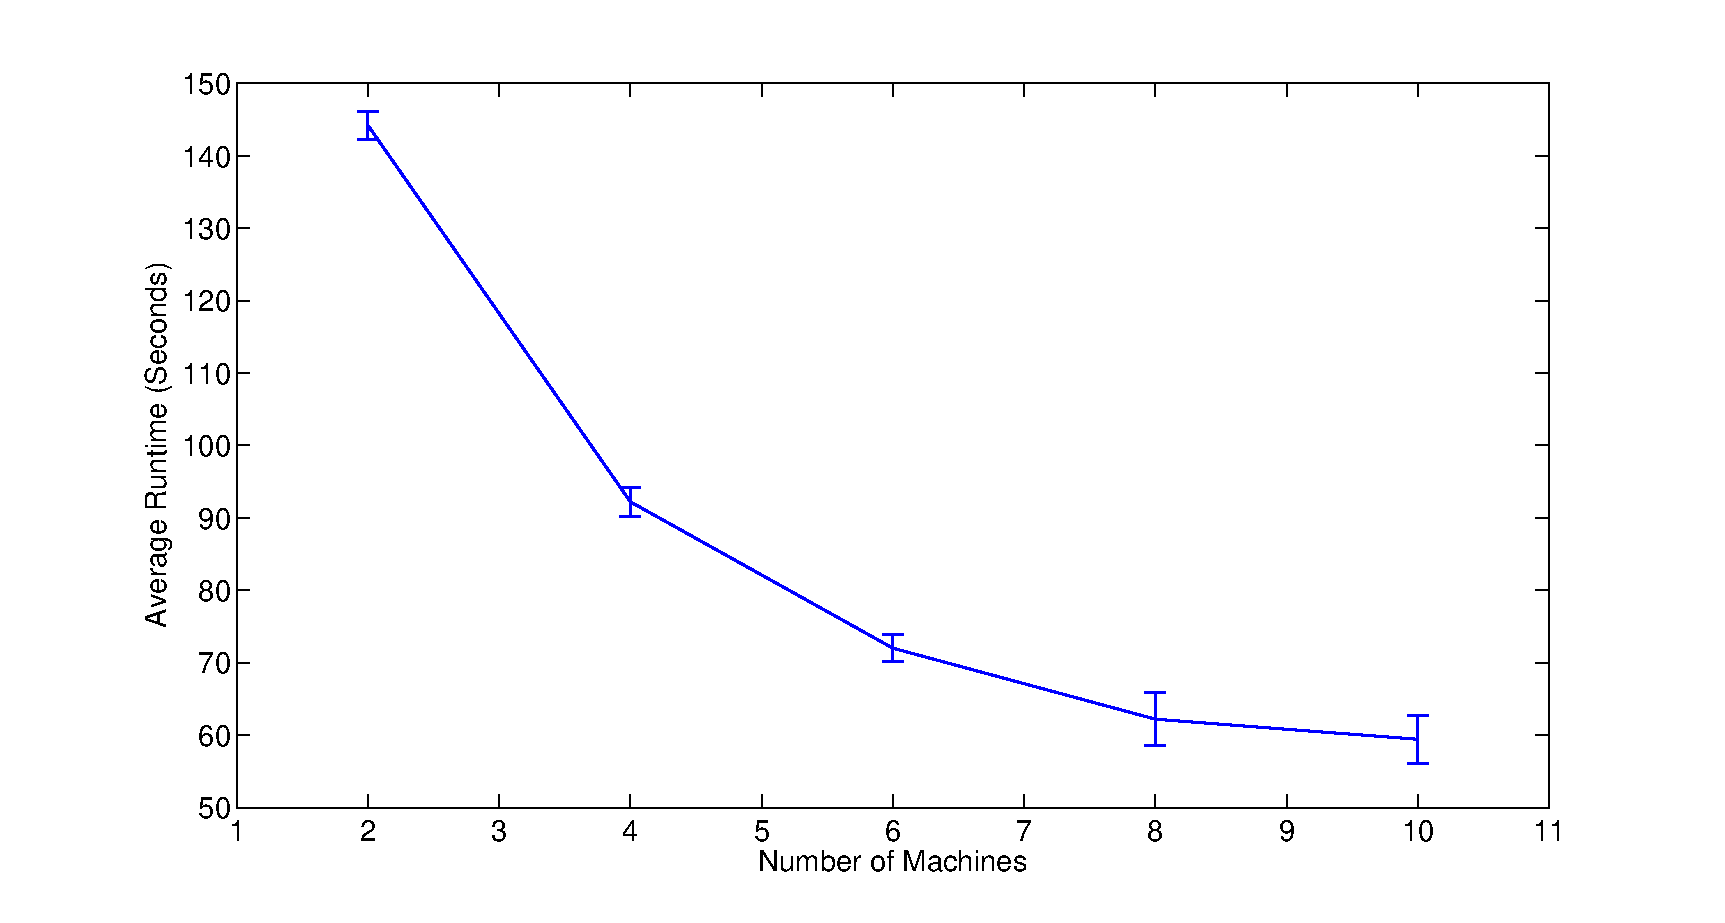
\includegraphics[scale=0.6]{resources/StratRLG.eps}
	\caption{Stratosphere Reverse Link Graph Runtime}
	\label{stratRLGRuntime}
\end{figure}

The Stratosphere implementation also shows the expected speed increase as extra nodes are added to the cluster. As with the Hadoop implementation, it begins to suffer from Amdahl's law towards the higher number of nodes in the cluster. Unlike with the Hadoop implementation, running the experiment on 10 machines does not increase the runtime, but the performance enhancement from adding more nodes clearly diminishes as the cluster gets larger. 

\begin{figure}[H]
	\centering
	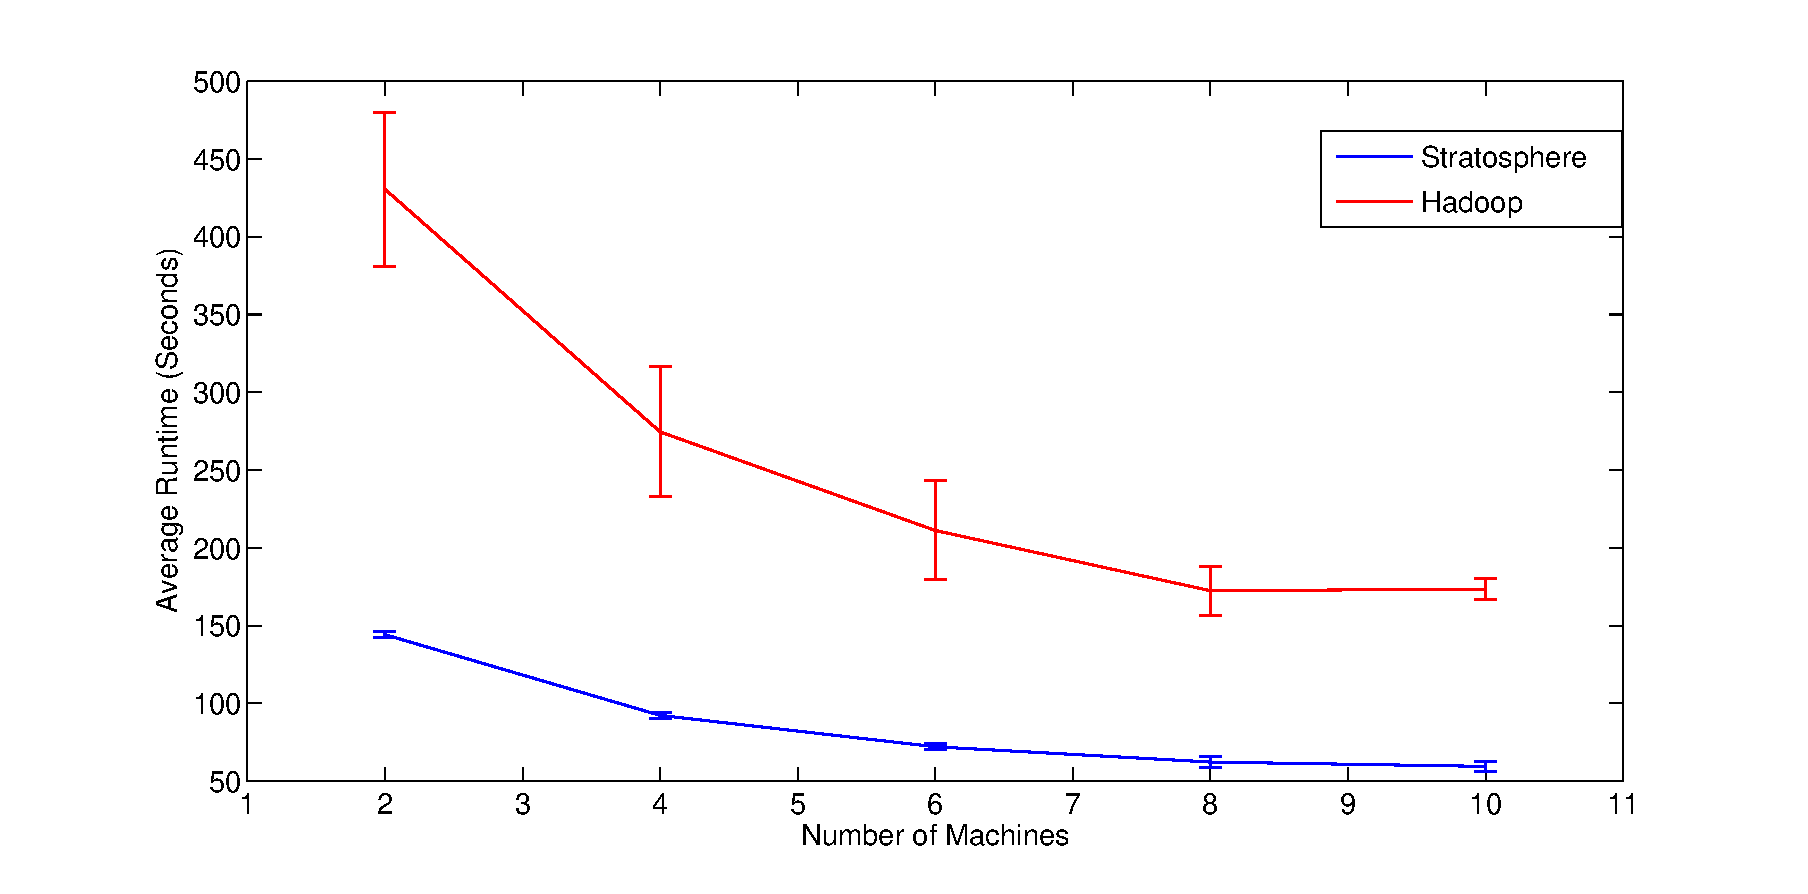
\includegraphics[scale=0.6]{resources/HadoopVStratRLG.eps}
	\caption{Comparison of Hadoop and Stratosphere Reverse Link Graph Runtime}
	\label{hadoopvstratRLGRuntime}
\end{figure}

When comparing runtime of the Hadoop and Stratosphere Reverse Link Graph implementations, it is clear that the Stratosphere experiment runs much faster across all cluster sizes. This contradicts the hypothesis, which expected that Hadoop would perform better for classic MapReduce problems. Potential reasons for this are explored in section \ref{Hypothesis Evaluation}.

In addition performing better, it appears that Stratosphere has a more predictable runtime. The standard deviation of Stratosphere experiments is much smaller, indicating that there is less variance in runtime. This may indicate that Stratosphere is less susceptible to the varying factors of the environment it is executing in, such as network congestion or disk usage.  

\begin{figure}[H]
	\centering
	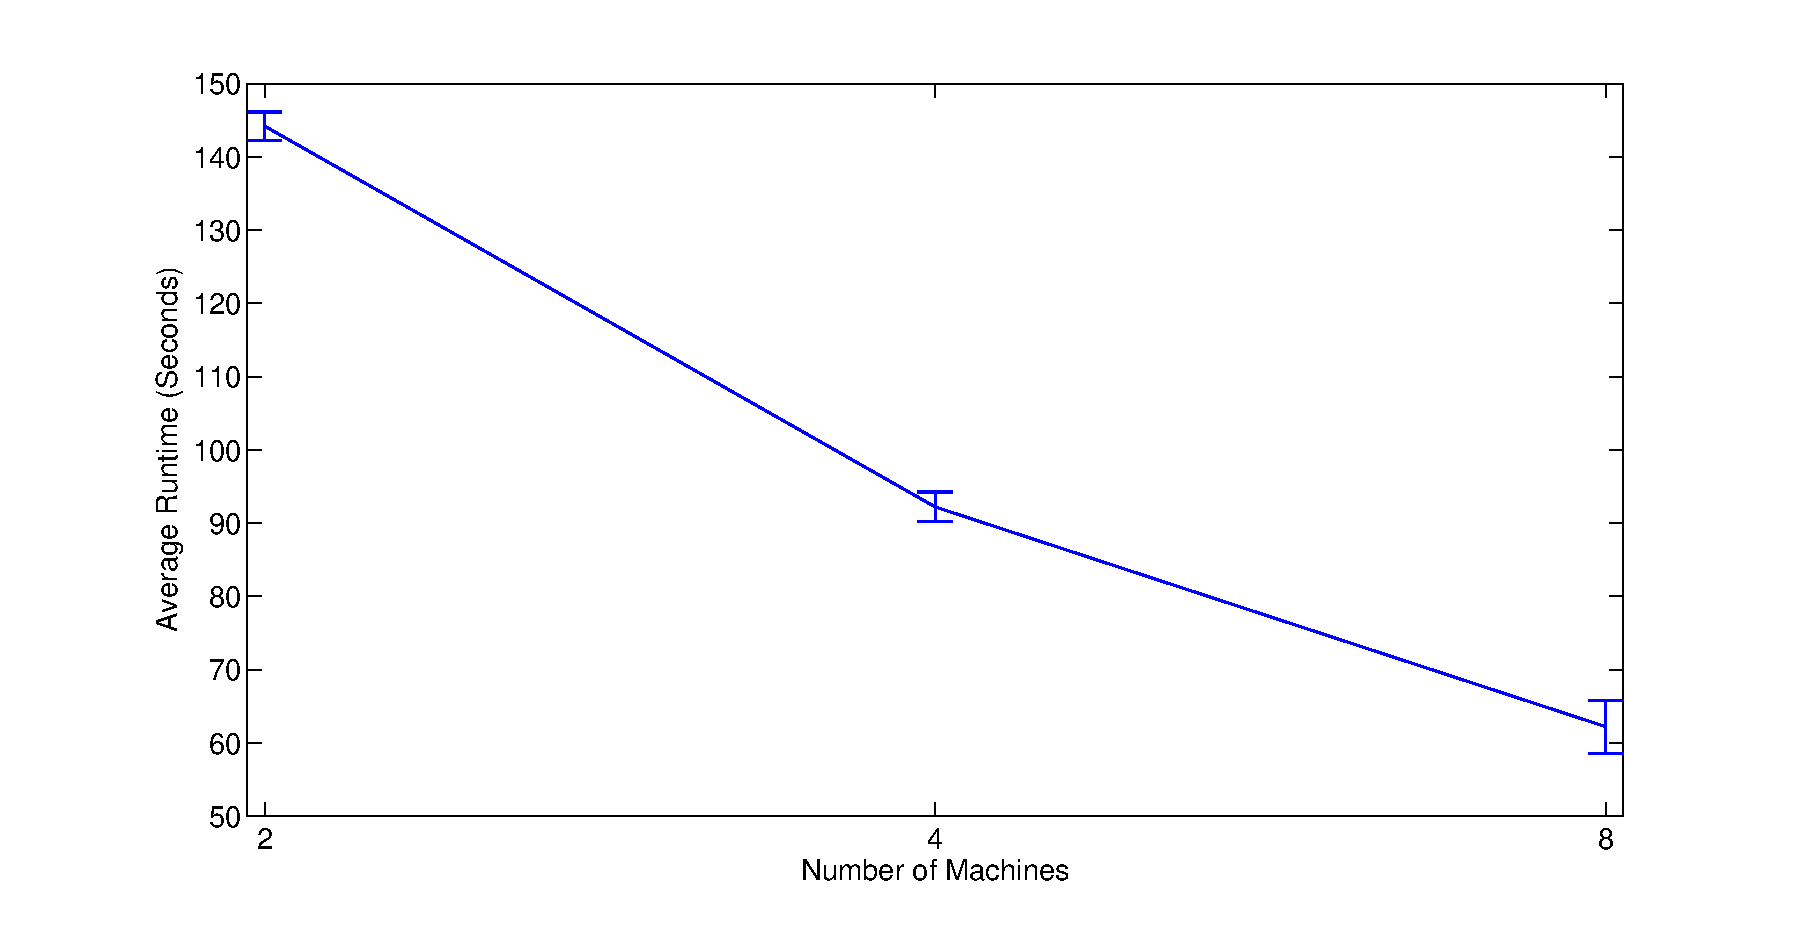
\includegraphics[scale=0.6]{resources/StratRLGScalability.eps}
	\caption{Logarithmic plot of Stratosphere Reverse Link Graph Runtime}
	\label{stratRLGScale}
\end{figure}

The Stratosphere implementation of Reverse Link Graph also scales near linearly to the amount of processors. When comparing to the Hadoop implementation, it appears that the implementation may scale slightly worse between 4 and 8 nodes, though this is likely to be because of the effects of Amdahl's law. Stratosphere would be more susceptible to the issues of parallel overhead as its runtime is lower, and communication would therefore take up a higher percentage of the overall execution time. 

\section{PageRank}

\subsection{Hadoop}
The Hadoop implementation of PageRank serves to show that the MapReduce paradigm is not capable of expressing all algorithms in an efficient manner. It clearly demonstrates a potent disadvantage of the MapReduce paradigm, and provides a point of comparison for the equivalent Stratosphere implementation.

Unfortunately, due to resource constraints on the cluster, it was not possible to compute the solution to PageRank using Hadoop on 2 or 4 nodes. This shows the ineffective nature of Hadoop when attempting to solve iterative problems. It also prevents an assessment of the scalability of the solution, as it was not possible to perform the task on half the number of nodes.

\begin{figure}[H]
\centering
	\begin{tabular}{lrr}
		\toprule
		Number of Machines & Average Runtime & Standard Deviation \\
		\midrule

		6 & 3429 & 150.58 \\
		8 & 3197 & 132.86 \\
		10 & 3060 & 117.06 \\
		\bottomrule
	\end{tabular}
	\caption{Hadoop PageRank Raw Data}
\end{figure}

\begin{figure}[H]
	\centering
	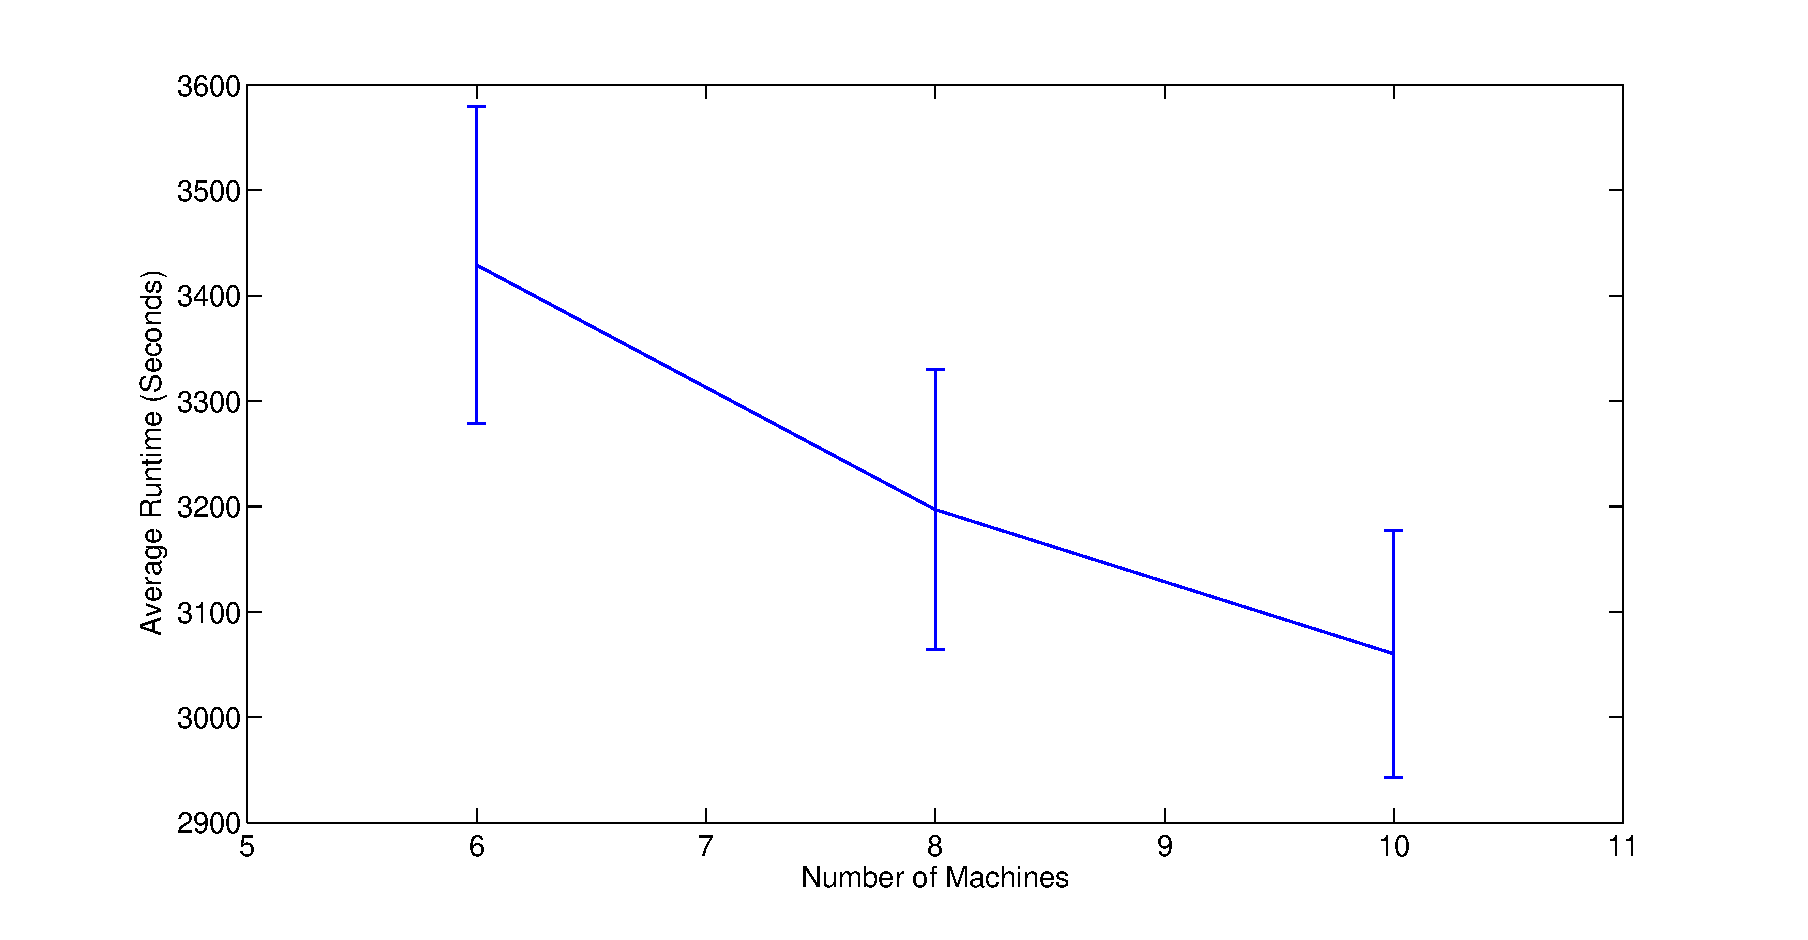
\includegraphics[scale=0.6]{resources/HadoopPR.eps}
	\caption{Hadoop PageRank Runtime}
\end{figure}

Despite using the same dataset, PageRank is much less efficient to compute in Hadoop than the Reverse Link Graph is. This can be seen clearly in figure \ref{hadoopRLGvPR}. Whilst it can be expected that PageRank will take longer to compute (with the Reverse Link Graph being a component of PageRank) the size of the difference shows that Hadoop is sub-optimal when performing iterative algorithms. A large part of this is that each iteration is implemented as a number of Map and Reduce steps. There is overhead for every MapReduce job submitted to Hadoop, as it must schedule the work across nodes, load the appropriate data, perform the computation and write the intermediate data to disk before moving on to the next step in the process. The overhead of this process would be less significant where larger data sizes are used, but would increase as more iterations were used (requiring more Map and Reduce steps), and as the cluster size increases (increasing the associated start up time). 

\begin{figure}[H]
	\centering
	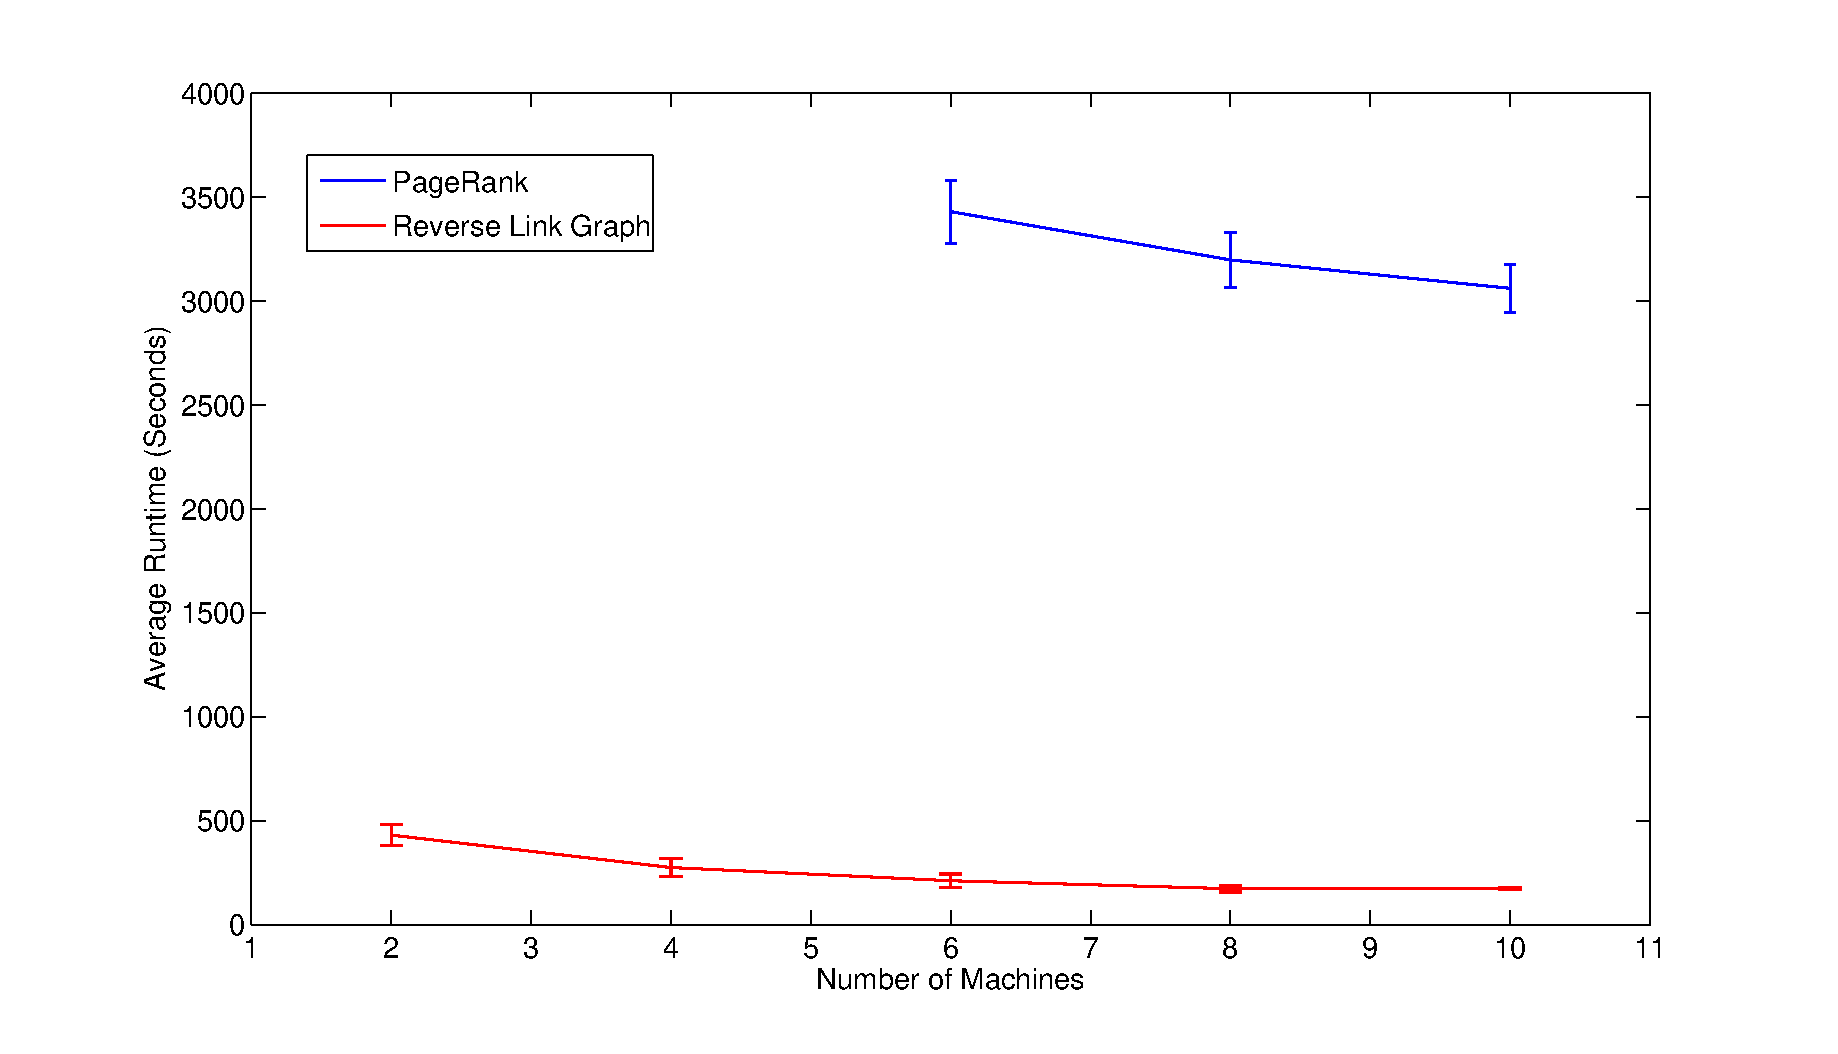
\includegraphics[scale=0.6]{resources/HadoopRLGvPR.eps}
	\caption{Hadoop PageRank and Reverse Link Graph Runtime Comparison}
	\label{hadoopRLGvPR}
\end{figure}

\subsection{Stratosphere}
The Stratosphere implementation of the PageRank algorithm shows the performance increases that are possible when using a more generalised paradigm such as PACT over MapReduce.  

\begin{figure}[H]
\centering
	\begin{tabular}{lrr}
		\toprule
		Number of Machines & Average Runtime & Standard Deviation \\
		\midrule

		2 & 588.00 & 0.57 \\
		4 & 565.66 & 2.51 \\
		6 & 553 & 2.64 \\
		8 & 533.66 & 2.08 \\
		10 & 522.00 & 2.64 \\
		\bottomrule
	\end{tabular}
	\caption{Hadoop PageRank Raw Data}
\end{figure}

\begin{figure}[H]
	\centering
	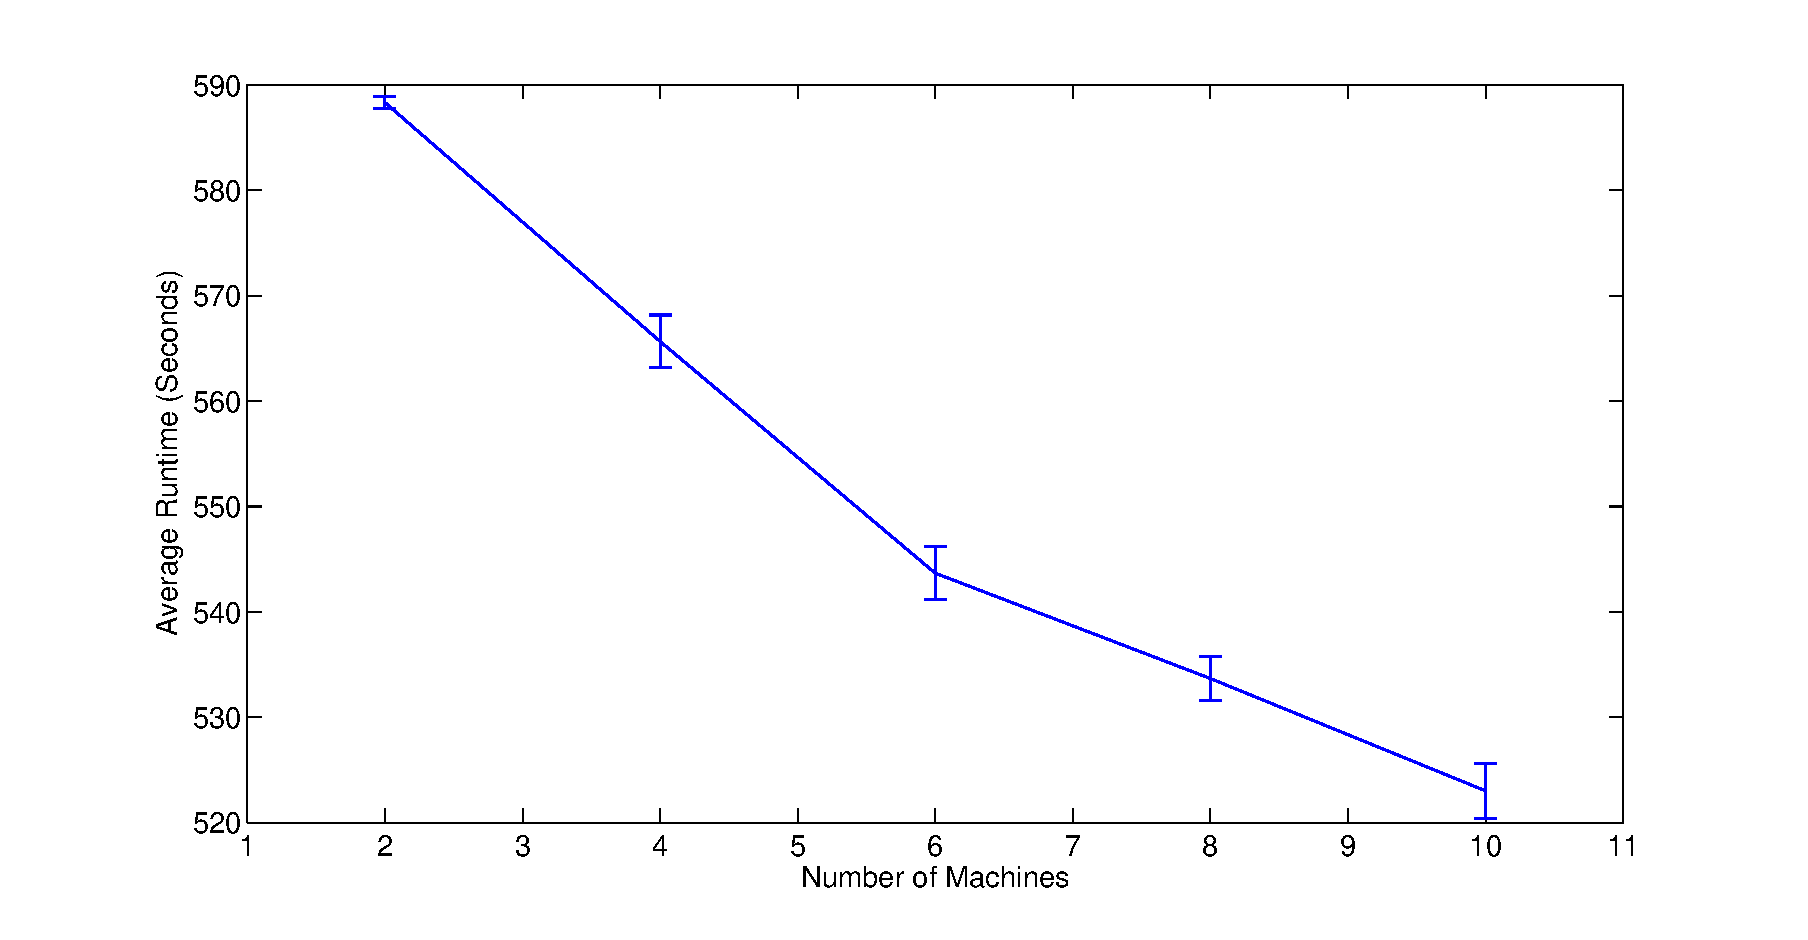
\includegraphics[scale=0.6]{resources/StratPR.eps}
	\caption{Stratosphere PageRank Runtime}
	\label{stratPR}
\end{figure}

The Stratosphere runtime performs significantly better than Hadoop when performing PageRank. In addition from benefiting from superior runtime in simple MapReduce cases (as show by the earlier experiments), Stratosphere benefits from having built-in support for iterations, and the ability to create complex Directed Acyclic Graphs representing the operations which must be carried out. This benefits Stratosphere as intermediate results can be stored in memory, and data does not necessarily have to be shuffled before subsequent processing steps can begin. This reduction in I/O and network overhead play a large role in improving the runtime performance of the experiment.

\begin{figure}[H]
	\centering
	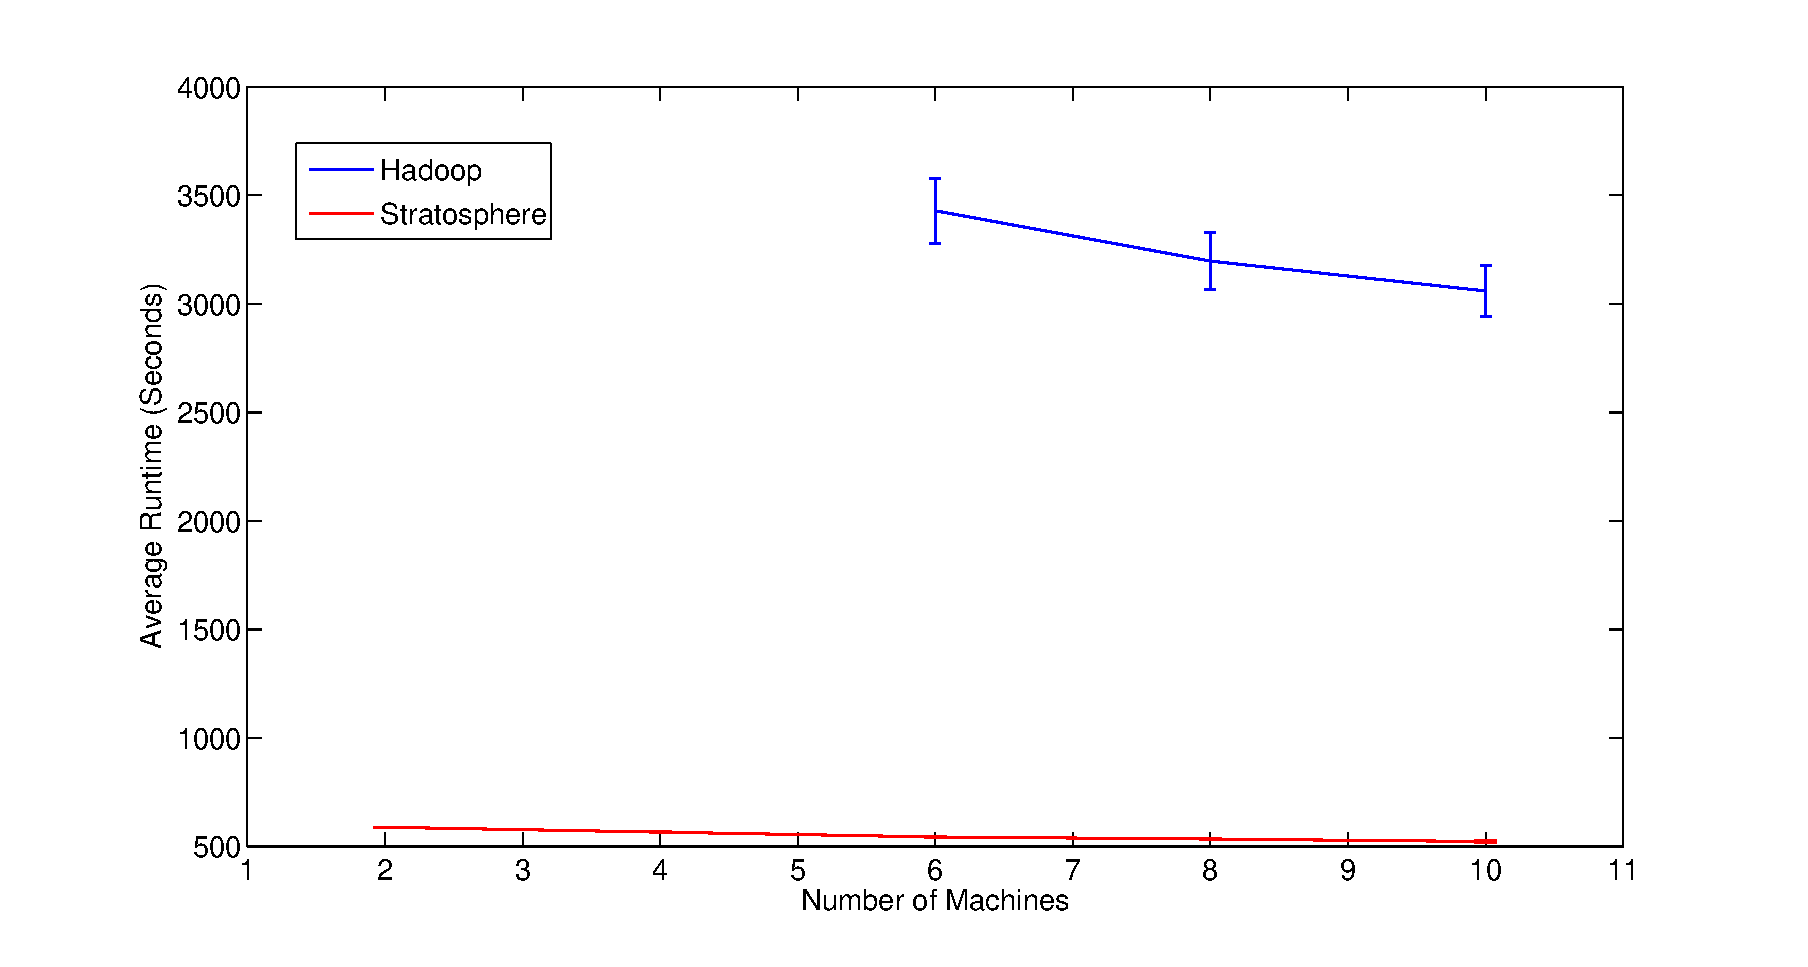
\includegraphics[scale=0.6]{resources/HadoopVStratPR.eps}
	\caption{Comparison of Hadoop and Stratosphere PageRank Runtime}
	\label{hadoopvstratpr}
\end{figure}

Unlike previous experiments, the Stratosphere PageRank implementation appears to handle the additional 2 machines from 4 to 6 in a similar manner to the improvement from 2 to 4 nodes. This is due to the poor speedup observed when extra nodes were added to the cluster. This behaviour can also be seen when adding machines to the Hadoop cluster, and we can therefore surmise that this is due to the nature of the problem, rather than an inherent behaviour of the runtime. 

\begin{figure}[H]
	\centering
	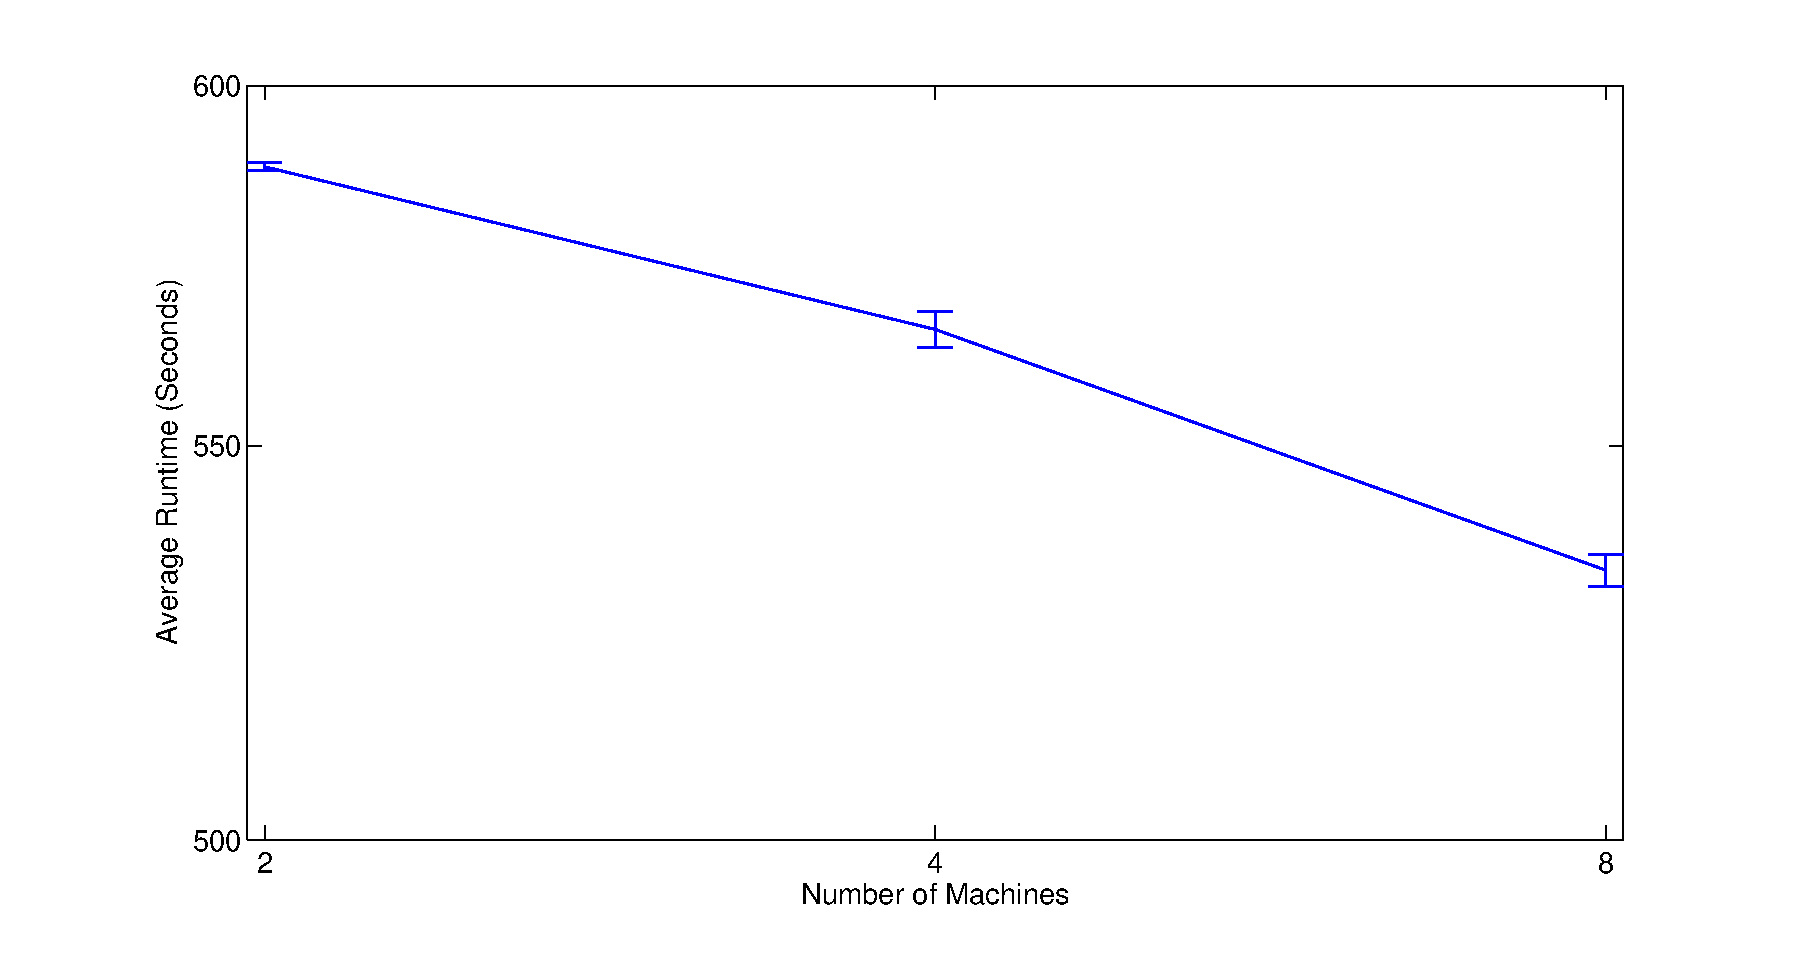
\includegraphics[scale=0.6]{resources/StratPRScalability.eps}
	\caption{Logarithmic Plot of Stratosphere PageRank Runtime}
\end{figure}

\section{Hypothesis Evaluation}
\label{Hypothesis Evaluation}
The hypothesis formed in the Experiment Design consisted of 3 core statements which summarised the expected outcome of the experiments.

\subsection{Hadoop outperforms Stratosphere in MapReduce Tasks}
It was expected that Hadoop would outperform Stratosphere when the data processing job was one which could inherently be expressed in a MapReduce manner. This part of the hypothesis was disproved, as Stratosphere performed consistently better when computing the Reverse Link Graph. After further analysis, there are various reasons why Stratosphere may perform better.

As indicated in previous research \cite{warneke2011exploiting}\cite{battre2010socc} Stratosphere writes to disk less than Hadoop, with disk I/O typically being a bottleneck in this type of task. Stratosphere is also more likely to utilise nodes fully, using upwards of 80\% of each machines CPU. Hadoop is more likely to allow system resources to be idle. 

Perhaps the largest reason behind the difference in runtime is that Stratosphere is capable of running each step of the computation in parallel. Whilst Hadoop will begin copying the data from Mappers as they complete, the actual Reduce logic will not be executed until all Mappers have finished execution \cite{white2009hadoop}. In contrast, Stratosphere will begin the Reduce step as soon as there is data and computing resources available.

\subsection{PACT improves upon MapReduce}
It was hypothesised that PACT would improve upon the core shortcomings of the MapReduce paradigm, by performing better at iterative algorithms.

The results of the Hadoop PageRank experiment clearly indicate that MapReduce is performs significantly worse at iterative algorithms than with other problems, due to the poor runtime in comparison with the Hadoop Reverse Link Graph experiment (despite using the same data). This indicates a problem with the broader MapReduce paradigm. 

Stratosphere performs significantly better than Hadoop at computing the PageRank. This is in a large part due to PACT; it is greatly supported by having support for iterations without having to write to disk, and without having to submit several processing jobs to complete one logical task. Having a more expressive range of operations is also clearly to PACTs advantage. In the PageRank experiment, Stratosphere benefited from having a dedicated Join operation rather than having to use a Map and a Reduce. 

\subsection{Hadoop and Stratosphere scale near-linearly}
The final statement in the hypothesis was that Hadoop and Stratosphere would scale in similar terms, both near-linearly. When considering scalability, an important metric is parallel speedup, which can be defined as the following formula:

$$S_{p} = \frac{T_{1}}{T_{p}}$$

In the case of tools such as Hadoop and Stratosphere, it is difficult to get a `serial time', as it would be artificial to run experiments on one node. This would be unreliable as the technologies are designed for use in clusters of machines, and there is therefore no clear definition of `serial runtime'. However, we can use the concept of speedup to measure how well the data processing tools scale, by simply comparing the average runtime with that of experiment run on half the number of nodes. For example

$$ S_{4} = \frac{T_{2}}{T_{4}} $$

Should the data scale perfectly (i.e. linearly), this value would always be $2$, as runtime would half as the processor count doubles. 

When this is calculated for the Reverse Link Graph experiment it yields the following results. As there is not a complete set of results for the PageRank experiment, it will not be considered.

\begin{figure}[H]
\centering
	\begin{tabular}{lrr}
		\toprule
		Number of Processors & Hadoop Speedup & Stratosphere Speedup\\
		\midrule

		4 & 1.568 & 1.592\\
		8 & 1.563 & 1.482 \\
		\bottomrule
	\end{tabular}
	\caption{Reverse Link Graph Speedup}
\end{figure}

This indicates that the hypothesis is correct. With both Hadoop and Stratosphere the algorithms get roughly $75\%$ faster when the processor count doubles. This is sub-linear (i.e. not $100\%$) owing to communication overhead, and other inherently serial factors in execution. As with all parallel algorithms, there is a point at which the serial cost of adding new nodes outweighs the benefit they give to the computation. This process is clear with Stratosphere as the number of processors increases, as the runtime is shorter causing serial elements to take up a greater proportion of the computation.

\section{Conclusion}
Several experiments have been designed and performed with the aim of determining whether Stratosphere can perform better than Hadoop, and whether the generalised execution framework that PACT provides has any real benefits of Hadoop. 

The results of these experiments have shown that Stratosphere outperforms Hadoop in cases where a problem both can and cannot be clearly expressed as MapReduce problem, with PACT playing a key role in enabling these performance improvements. 

Whilst this indicates that Stratosphere is a more efficient tool in the general case for large scale data processing, there are several other considerations that should be made when choosing a tool for real-world applications.